\documentclass[aspectratio=169]{beamer}

\usetheme{Madrid}
\usecolortheme{default}
\setbeamertemplate{navigation symbols}{}
\setbeamertemplate{footline}[frame number]
\setbeamercovered{transparent}

\usepackage[utf8]{inputenc}
\usepackage[spanish]{babel}
\usepackage{graphicx}
\usepackage{booktabs}
\usepackage{multirow}
\usepackage{amsmath}
\usepackage{amssymb}
\usepackage{subcaption}
\usepackage{tikz}
\usetikzlibrary{positioning,arrows.meta,shapes.geometric}

\graphicspath{{../imagenes/}{../imagenes/Posibles img/}}

\title[TFT para el Costo Marginal del SEN]{Estimación del Costo Marginal en el SEN mediante Temporal Fusion Transformer: Comparación de Estrategias de Variables Exógenas, Arquitecturas y Cuantificación de Incertidumbre}
\author[E. B. Mitchell García]{Edward Benjamín Mitchell García}
\institute[DIM, FCFM, U. de Chile]{
    Departamento de Ingeniería Matemática \\
    Facultad de Ciencias Físicas y Matemáticas \\
    Universidad de Chile \\[1em]
    \small Profesor guía: Alejandro Jofré Cáceres
}
\date{2026}

\begin{document}

% ============================================================
\begin{frame}
    \titlepage
\end{frame}

\begin{frame}{Contenidos}
    \tableofcontents
\end{frame}

% ============================================================
\section{Motivación y objetivos}

\begin{frame}{El SEN en transición}
    \begin{itemize}
        \item El Sistema Eléctrico Nacional (SEN) chileno ha experimentado una transición acelerada hacia generación solar: la participación ERNC pasó de $\sim$20\% a $\sim$40\% de la generación total desde 2020.
        \item Esto introduce \textbf{volatilidad estructural creciente} en el costo marginal horario: episodios de sobreoferta solar (\textit{curtailment}) y transiciones de precio abruptas al entrar/salir el bloque fotovoltaico.
        \item En 2024 se perdieron \textbf{5\,908,71\,GWh} de energía renovable por \textit{curtailment}, un aumento del \textbf{149\%} respecto al año anterior.
        \item Los métodos estadísticos clásicos (ARIMA, modelos de descomposición) capturan mal esta dinámica no lineal y cambiante.
        \item \textbf{Pregunta}: ¿puede un modelo híbrido de \textit{deep learning}, con una señal exógena simple y determinista, mejorar el pronóstico horario y cuantificar honestamente su incertidumbre?
    \end{itemize}
\end{frame}

\begin{frame}{Objetivos}
    \textbf{Objetivo general}
    \begin{itemize}
        \item Desarrollar y evaluar un modelo híbrido basado en Temporal Fusion Transformer (TFT) para el pronóstico horario del costo marginal en el SEN, con cuantificación de incertidumbre calibrada.
    \end{itemize}
    \vspace{0.5em}
    \textbf{Objetivos específicos}
    \begin{itemize}
        \item Comparar dos estrategias de \textit{features} exógenas: Prophet+Clima (P+C) vs.\ Sol+Clima (S+C).
        \item Comparar dos mecanismos de normalización del Transformer: LayerNorm vs.\ Dynamic Tanh.
        \item Proponer y evaluar LW-ACP, un método de Conformal Prediction que combina ponderación horaria con adaptación \textit{online}.
        \item Caracterizar mecanísticamente los errores más extremos del modelo.
    \end{itemize}
\end{frame}

% ============================================================
\section{Datos}

\begin{frame}{Datos}
    \begin{itemize}
        \item Fuente: Coordinador Eléctrico Nacional (CEN) de Chile.
        \item Variable objetivo: costo marginal horario, enero 2020 -- abril 2026 ($\sim$55\,000 obs.\ por barra).
        \item Ocho barras de 220\,kV, seleccionadas por representatividad geográfica:
        \begin{itemize}
            \item Norte (solar/eólico): Atacama, Cardones, Crucero, Pan de Azúcar, Tarapacá
            \item Centro: Quillota
            \item Sur (hidroeléctrico): Charrúa, Puerto Montt
        \end{itemize}
        \item División temporal estricta: 70\% entrenamiento / 15\% validación / 15\% prueba, respetando causalidad.
    \end{itemize}
\end{frame}

\begin{frame}{Serie de costo marginal por barra}
    \centering
    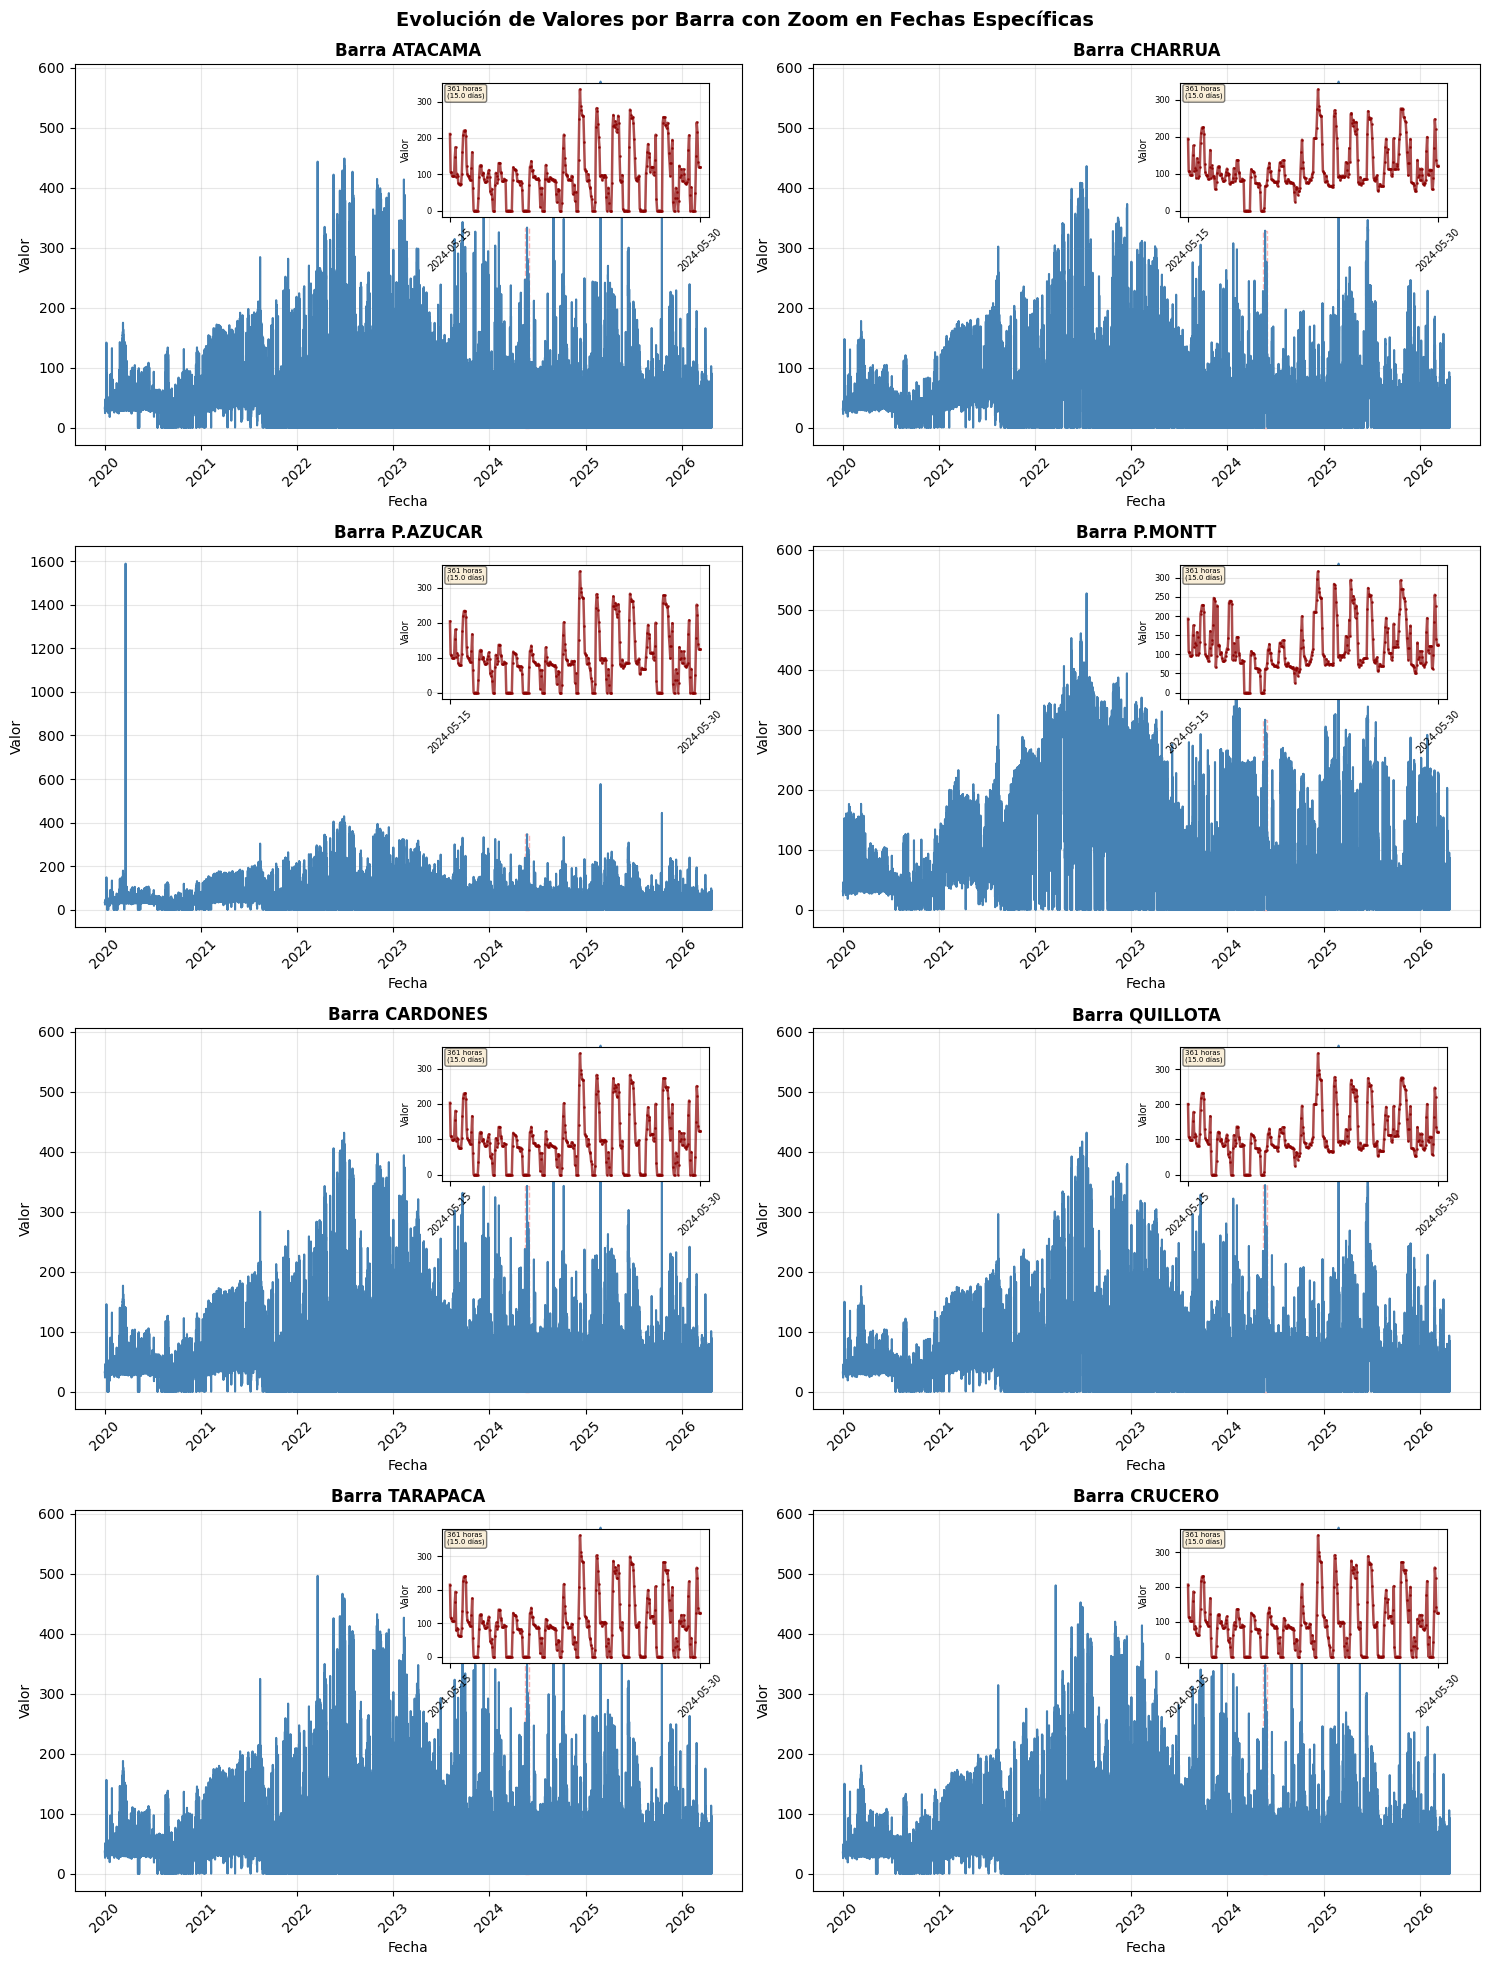
\includegraphics[width=\textwidth,height=0.82\textheight,keepaspectratio]{Serie Barras.png}
\end{frame}

% ============================================================
\section{Metodología}

\begin{frame}[fragile]{Pipeline general}
    \centering
    \begin{tikzpicture}[
        scale=0.74, every node/.style={scale=0.74},
        box/.style={rectangle, draw, thick, rounded corners, align=center, minimum height=1.05cm, text width=3.2cm, font=\small},
        arr/.style={-{Stealth[length=2mm]}, thick}
    ]
        \node[box, fill=blue!8]                        (datos)    at (0,0)    {Datos CEN\\(8 barras, 2020--2026)};
        \node[box, fill=blue!8]                        (prepro)   at (0,-1.6) {Preprocesamiento\\(outliers, clima, posición solar)};

        \node[box, fill=orange!12]                     (pc)       at (-2.6,-3.4) {P+C\\Prophet + TFT};
        \node[box, fill=orange!12]                     (sc)       at (2.6,-3.4)  {S+C\\TFT único};

        \node[box, fill=orange!12]                     (stacking) at (-2.6,-5.0) {Stacking\\Optimization};

        \node[box, fill=green!10, text width=4.4cm]    (pred)     at (0,-6.8) {Predicción puntual ganadora\\(S+C-LN)};
        \node[box, fill=green!10]                      (cp)       at (0,-8.4) {Conformal Prediction\\(LW-ACP)};

        \draw[arr] (datos) -- (prepro);
        \draw[arr] (prepro) -- (pc);
        \draw[arr] (prepro) -- (sc);
        \draw[arr] (pc) -- (stacking);
        \draw[arr] (stacking.south) -- ++(0,-6mm) -| (pred.north west);
        \draw[arr] (sc.south) -- ++(0,-6mm) -| (pred.north east);
        \draw[arr] (pred) -- (cp);
    \end{tikzpicture}
    \vspace{0.5em}

    \textit{Todos los modelos se entrenan de forma independiente por barra.}
\end{frame}

\begin{frame}{Dos estrategias de \textit{features} exógenas}
    \begin{columns}
        \column{0.48\textwidth}
        \textbf{P+C: Prophet + Clima}
        \begin{itemize}
            \item Prophet descompone la serie en tendencia + estacionalidad.
            \item El TFT modela tanto el precio como el residuo de Prophet.
            \item Stacking Optimization combina ambas predicciones.
        \end{itemize}
        \column{0.48\textwidth}
        \textbf{S+C: Sol + Clima}
        \begin{itemize}
            \item Reemplaza la descomposición de Prophet por variables de posición solar (elevación, coseno de elevación) calculadas de forma \textbf{determinista} vía \texttt{pvlib}.
            \item Una única instancia del TFT, sin Stacking.
            \item Más simple: no requiere ajustar Prophet ni un segundo modelo de residuos.
        \end{itemize}
    \end{columns}
\end{frame}

\begin{frame}{Temporal Fusion Transformer}
    \begin{itemize}
        \item Arquitectura de \textit{deep learning} para forecasting de series de tiempo con atención interpretable (Lim et al., 2021).
        \item Ventana de contexto: 168 horas (1 semana). Horizonte principal: $h=1$ hora.
        \item Se entrena minimizando MAE directamente (no la pérdida cuantílica original del TFT), dejando la cuantificación de incertidumbre a Conformal Prediction.
        \item Se comparan dos mecanismos de normalización interna:
        \begin{itemize}
            \item \textbf{LayerNorm (LN)}: normalización local, por paso temporal.
            \item \textbf{Dynamic Tanh (DyT)}: un único escalar $\alpha$ global aprendido, sin normalización explícita.
        \end{itemize}
    \end{itemize}
\end{frame}

\begin{frame}{Curvas de aprendizaje}
    \centering
    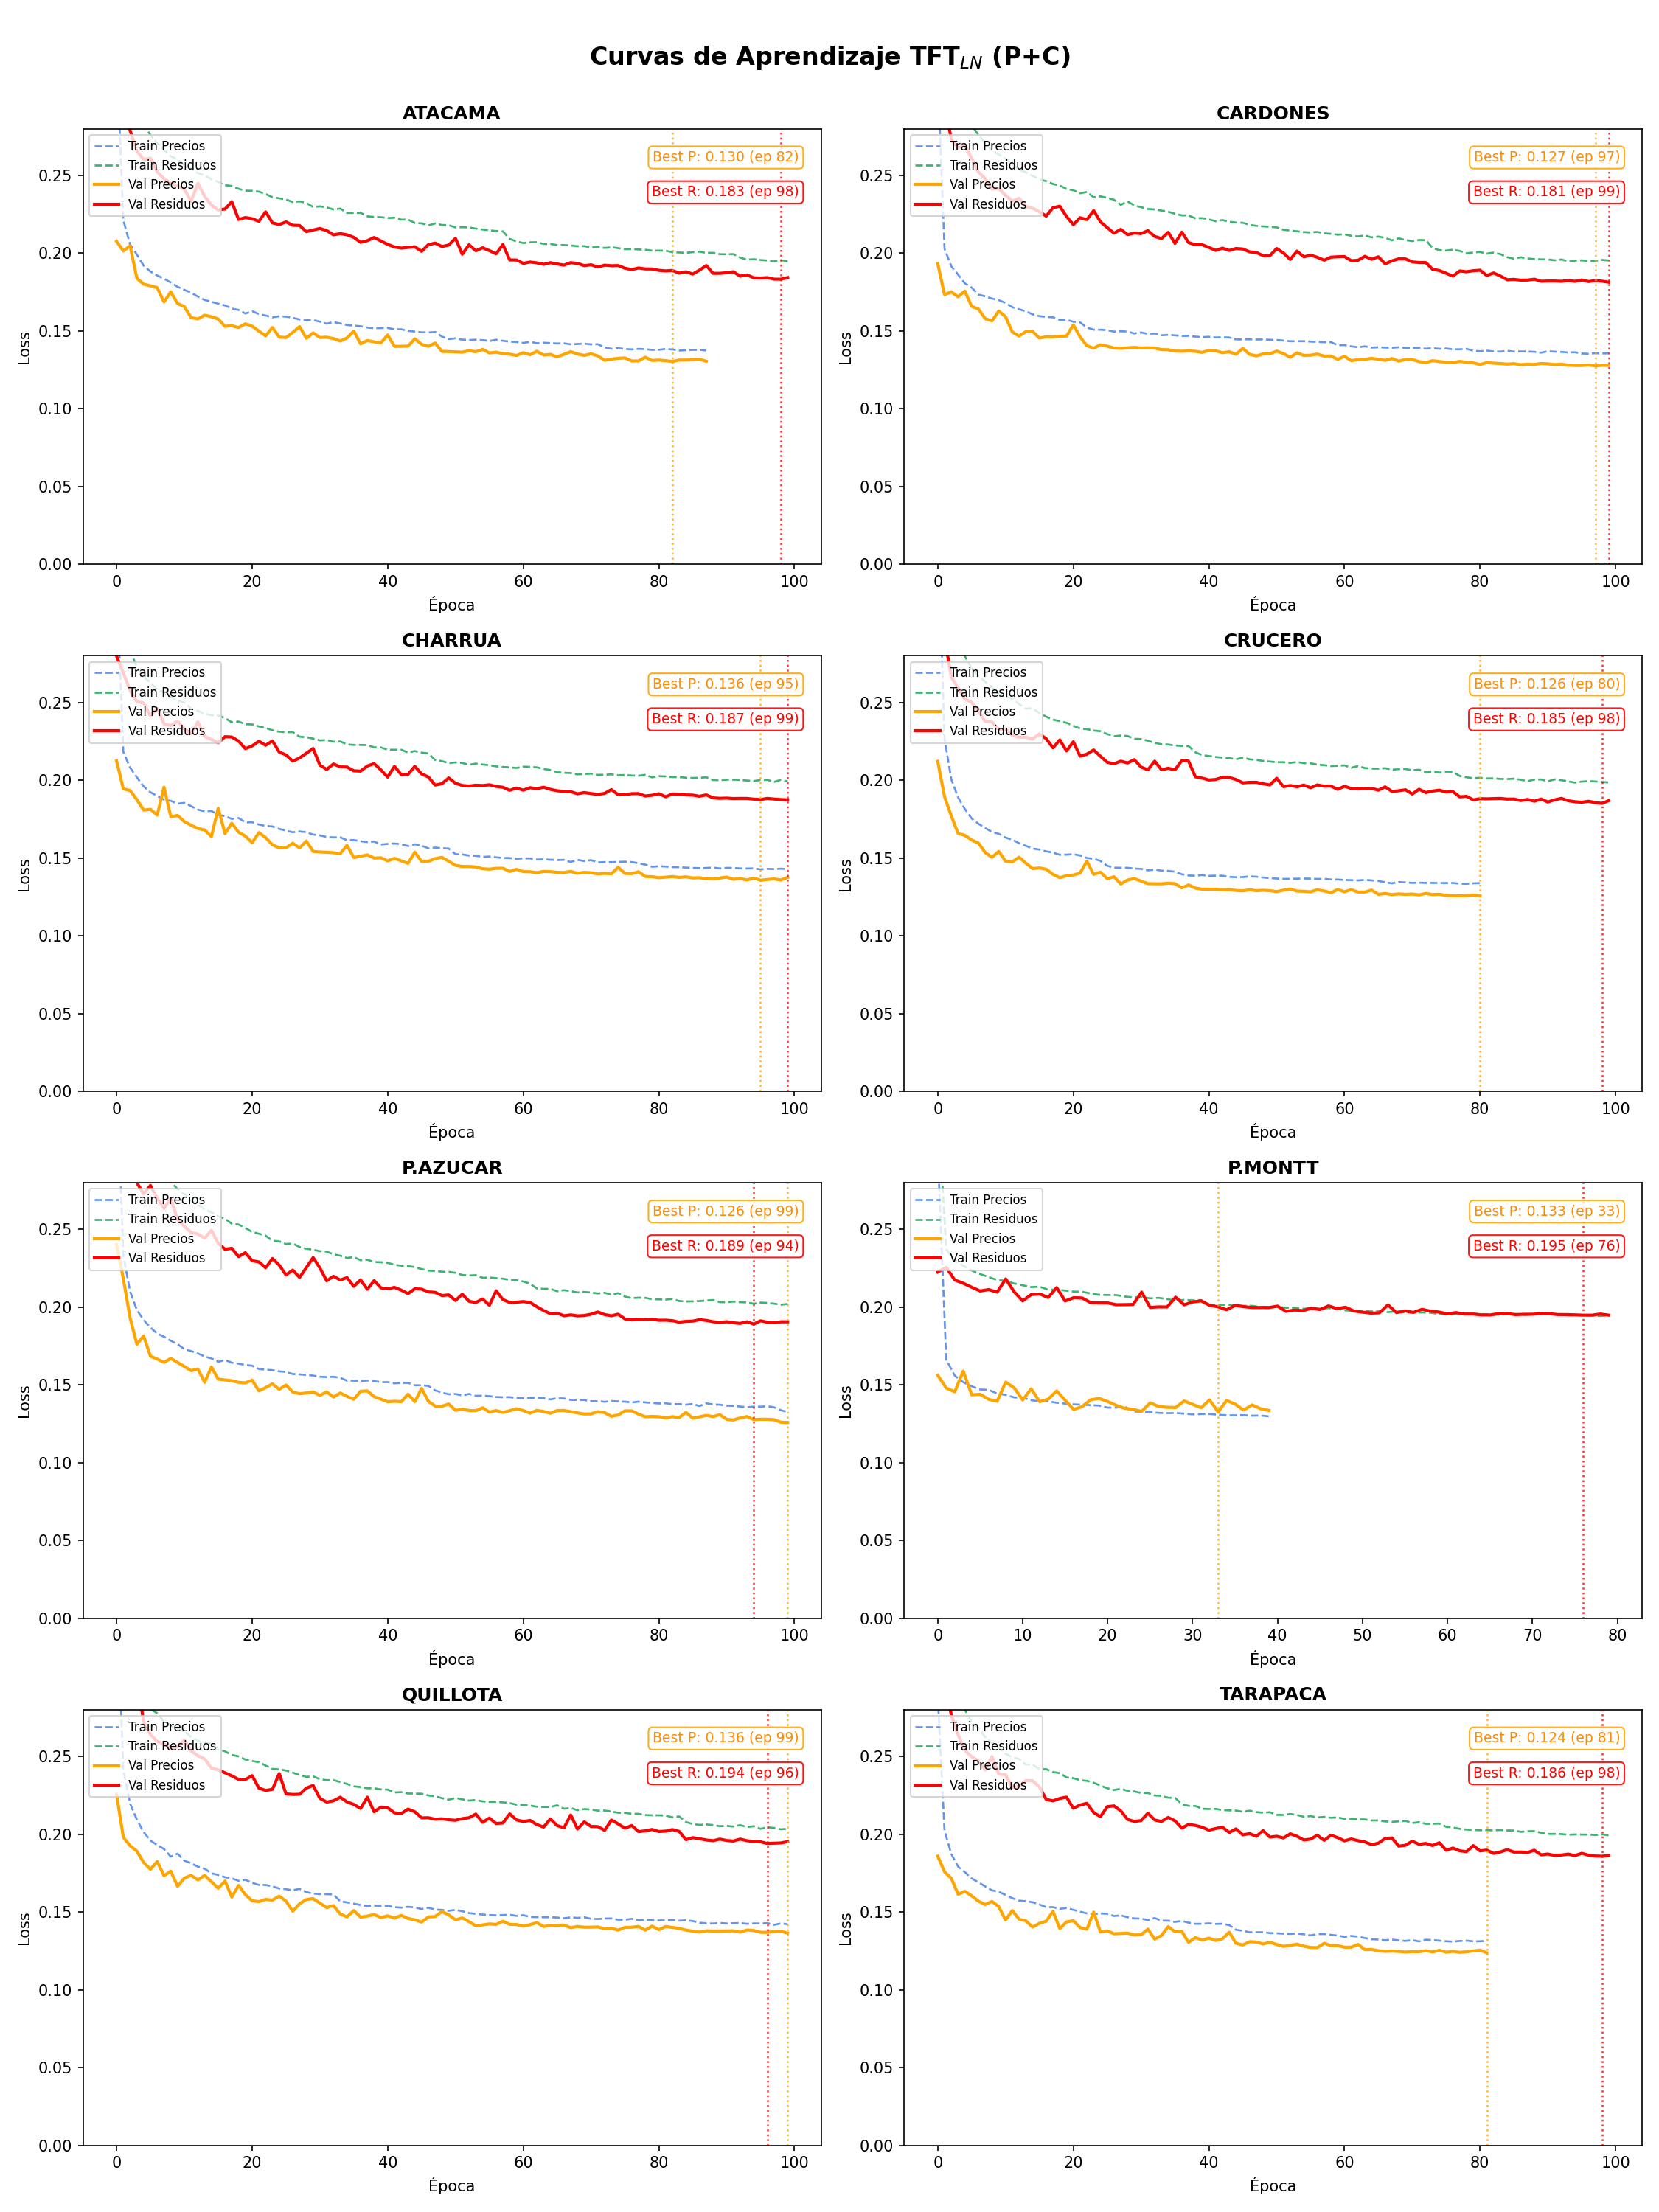
\includegraphics[width=\textwidth,height=0.82\textheight,keepaspectratio]{Curvas Aprendizaje LN.png}
\end{frame}

\begin{frame}{Conformal Prediction: de Split CP a LW-ACP}
    \centering
    \textbf{Split CP} $\;\longrightarrow\;$ \textbf{ACI} $\;\longrightarrow\;$ \textbf{LW-ACP}
    \vspace{1em}
    \begin{itemize}
        \item \textbf{Split CP} (clásico): un cuantil fijo $q$, calculado una vez sobre calibración.
        \item \textbf{ACI} (Gibbs \& Candès, 2021): adapta el nivel de cobertura $\alpha_t$ \textit{online} según los aciertos/fallos recientes.
        \item \textbf{LW Split CP}: normaliza el \textit{score} de no conformidad por la desviación estándar de cada hora del día $\hat\sigma_h$ (heterocedasticidad horaria).
        \item \textbf{LW-ACP (contribución de este trabajo)}: combina ambos mecanismos (ponderación horaria \emph{y} adaptación \textit{online}) en un solo método.
    \end{itemize}
\end{frame}

% ============================================================
\section{Resultados}

\begin{frame}{S+C supera a P+C}
    \begin{table}
        \centering
        \small
        \begin{tabular}{lcc}
            \toprule
             & \textbf{S+C mejor} & \textbf{Significativo (DM)} \\
            \midrule
            De 16 combinaciones (8 barras $\times$ 2 arq.) & 14 & 13 \\
            \bottomrule
        \end{tabular}
    \end{table}
    \vspace{1em}
    \begin{itemize}
        \item S+C, la estrategia más simple, supera a P+C en 14 de 16 combinaciones (13 estadísticamente significativas, test de Diebold-Mariano con varianza Newey-West).
        \item El análisis de interpretabilidad del TFT confirma que la posición solar domina el decoder en 6 de las 8 barras: el modelo efectivamente aprende a usar esa señal.
        \item Conclusión: la señal física de posición solar es al menos tan informativa como la descomposición estadística de Prophet, con menor complejidad de pipeline.
    \end{itemize}
\end{frame}

\begin{frame}{Interpretabilidad: importancia de variables en el decoder}
    \begin{itemize}
        \item El decoder de S+C-LN solo recibe las tres variables solares y el índice temporal relativo.
    \end{itemize}
    \begin{table}
        \centering
        \tiny
        \begin{tabular}{lrrrr}
            \toprule
            Barra & \texttt{elevacion\_solar} & \texttt{relative\_time\_idx} & \texttt{cos\_elevacion} & \texttt{es\_horario\_verano} \\
            \midrule
            Atacama       & 26.33 & 31.59 & 23.82 & 18.27 \\
            Cardones      & 27.72 & 41.78 & 21.02 &  9.47 \\
            Charrúa       & 33.04 & 40.35 &  9.29 & 17.32 \\
            Crucero       & 63.46 &  7.94 & 13.80 & 14.80 \\
            Pan de Azúcar & 44.28 & 20.43 & 15.30 & 19.99 \\
            Puerto Montt  & 16.86 & 44.77 & 30.04 &  8.33 \\
            Quillota      & 46.88 & 12.25 & 24.68 & 16.19 \\
            Tarapacá      & 39.25 & 29.94 &  9.84 & 20.97 \\
            \bottomrule
        \end{tabular}
    \end{table}
    \begin{itemize}
        \item Sumando \texttt{elevacion\_solar} + \texttt{cos\_elevacion}: la posición solar domina el decoder (42.3\%--77.3\%) en \textbf{6 de las 8 barras}.
        \item Puerto Montt es la excepción más clara: \texttt{relative\_time\_idx} lidera (44.8\%) por sobre la posición solar (16.9\%).
    \end{itemize}
\end{frame}

\begin{frame}{LayerNorm vs.\ Dynamic Tanh}
    \begin{table}
        \centering
        \small
        \begin{tabular}{lccc}
            \toprule
            & \textbf{Significativas (DM)} & \textbf{LN gana} & \textbf{Dif.\ típica} \\
            \midrule
            De 16 combinaciones & 12 & 11 de 12 & $<0.5$\,USD/MWh \\
            \bottomrule
        \end{tabular}
    \end{table}
    \vspace{0.5em}
    \begin{itemize}
        \item A una hora LN gana en 11 de 12 combinaciones significativas, pero la ventaja \textbf{no supera la variabilidad entre semillas ni se mantiene a 24 horas}: en la práctica, ambas son equivalentes.
        \item \textbf{Robustez a la semilla}: al repetir el entrenamiento con 5 semillas distintas, los intervalos de MAE de LN y DyT se solapan completamente en las 3 barras piloto.
        \begin{itemize}
            \item La ventaja de LN es del mismo orden de magnitud que la variabilidad de inicialización.
            \item No la contradice: el test DM compara errores pareados hora a hora dentro de una misma semilla, evidencia de un tipo distinto.
        \end{itemize}
    \end{itemize}
\end{frame}

\begin{frame}{Análisis de errores extremos: desfase de fase}
    \centering
    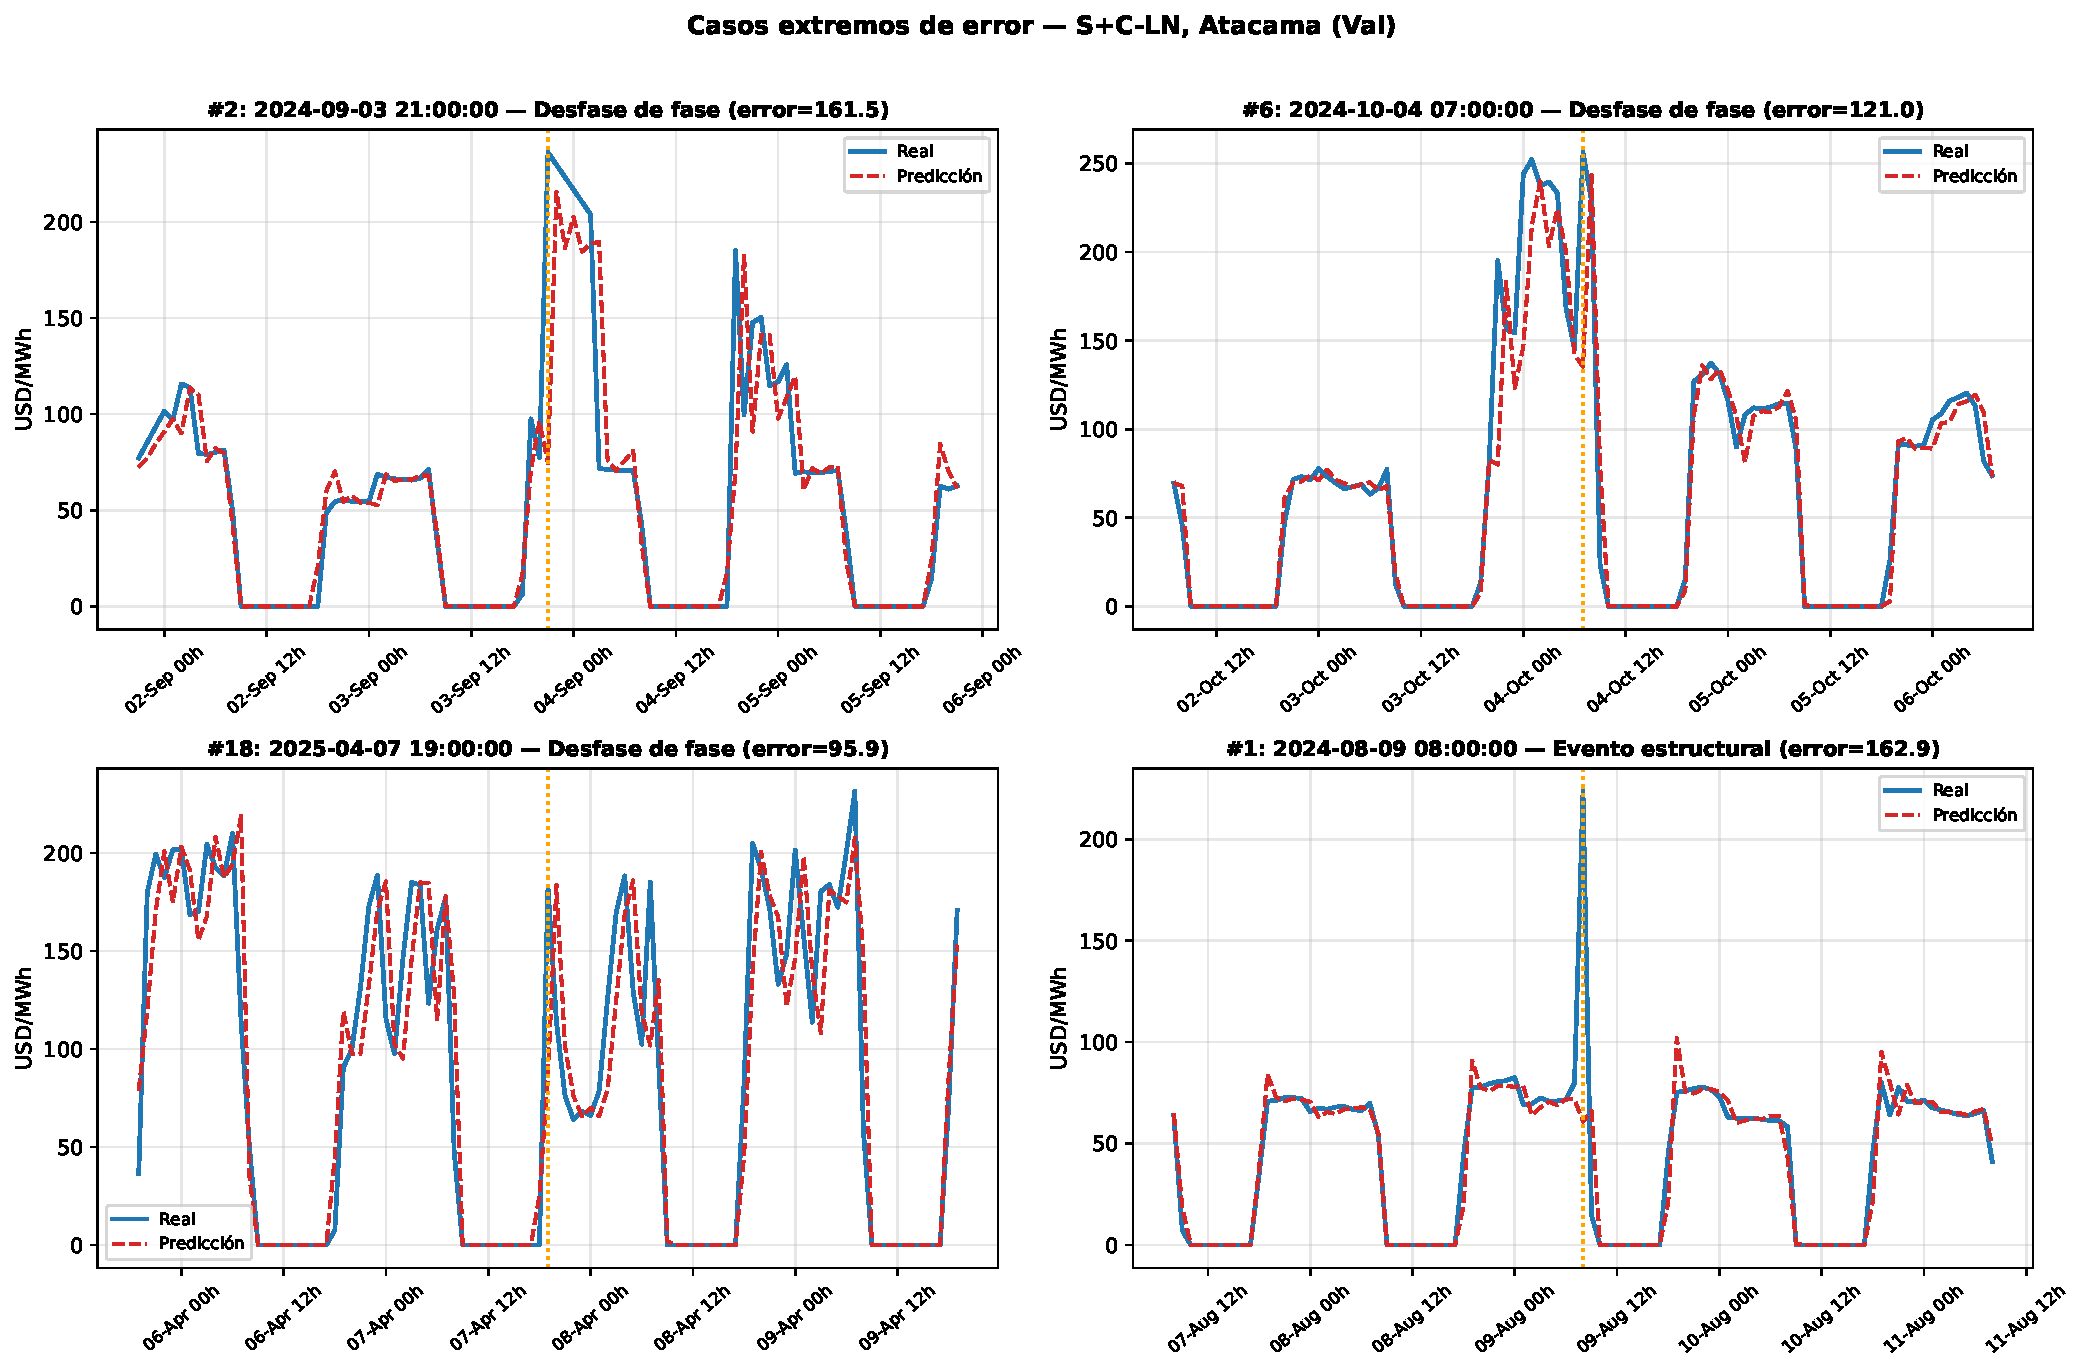
\includegraphics[width=0.72\textwidth]{fig_phase_shift_panel_2x2.pdf}
\end{frame}

\begin{frame}{Análisis de errores extremos: desfase de fase}
    \begin{itemize}
        \item Entre el 80\% y el 100\% de los veinte mayores errores de validación, en las ocho barras, corresponden a un \textbf{desfase de fase}: el modelo predice correctamente la magnitud de la transición diaria, pero con $\sim$1 hora de retraso.
        \item Patrón consistente en todo el SEN, no un artefacto de una barra particular.
        \item Errores de gran amplitud pero muy localizados en el tiempo $\Rightarrow$ motiva directamente el valor de Conformal Prediction adaptativo y ponderado por hora.
    \end{itemize}
\end{frame}

\begin{frame}{Puerto Montt: un caso no resuelto}
    \begin{itemize}
        \item Peor desempeño del sistema de forma consistente: MAE de prueba 13.68\,USD/MWh vs.\ 6.4--8.0\,USD/MWh del resto.
        \item Media y desviación estándar de precio sustancialmente mayores: dependencia hidrológica de baja frecuencia (meses), más lenta que la ventana de contexto del TFT (168h).
        \item Se probaron \textit{features} hídricas propias (cota del embalse, agua caída) en variantes H+C y S+H+C: \textbf{no lograron mejorar} sobre S+C.
        \item Puerto Montt también exhibe desfase de fase, pero no ligado al ciclo solar como el resto del SEN.
        \item Queda documentado como un caso estructuralmente distinto, no resuelto por las extensiones exploradas.
    \end{itemize}
\end{frame}

\begin{frame}{LW-ACP: ejemplo de intervalo}
    \centering
    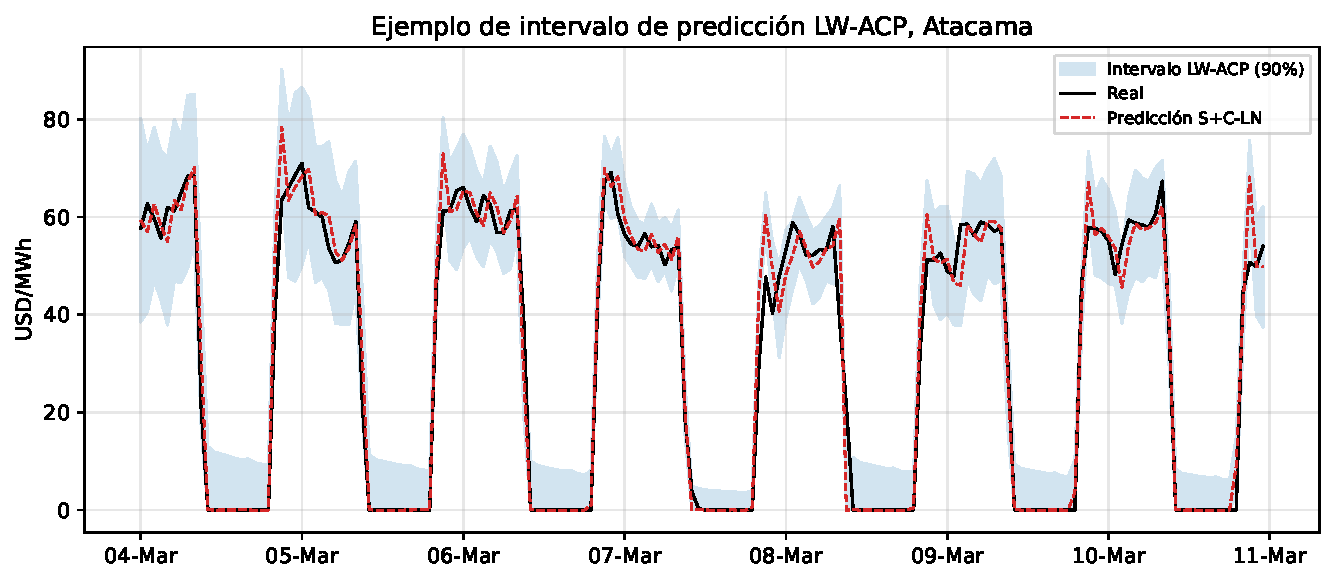
\includegraphics[width=0.95\textwidth]{fig_cp_ejemplo_intervalo.pdf}
\end{frame}

\begin{frame}{LW-ACP: cobertura y ancho por hora}
    \centering
    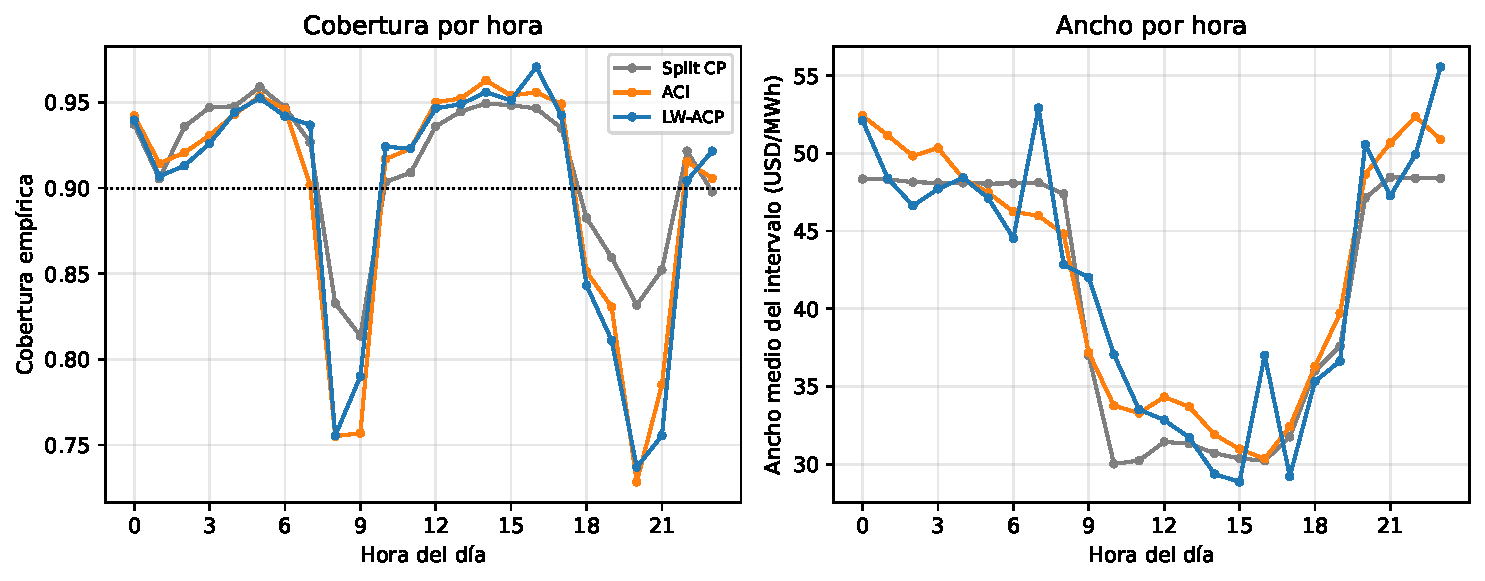
\includegraphics[width=0.95\textwidth]{fig_cp_cobertura_ancho_hora.pdf}
\end{frame}

\begin{frame}{Resultados de Conformal Prediction (90\% nominal)}
    \begin{table}
        \centering
        \small
        \begin{tabular}{lrrrr}
            \toprule
            \textbf{Método} & \textbf{Ancho} & \textbf{$|$Cob$-$0.90$|$} & \textbf{Winkler} & \textbf{Pinball} \\
            \midrule
            Split CP               & 40.90 & 0.0112 & 76.65 & 1.916 \\
            LW Split CP            & \textbf{40.69} & 0.0108 & 76.23 & 1.906 \\
            ACI ($\gamma=0.05$)    & 42.21 & \textbf{0.0023} & 72.31 & 1.808 \\
            LW-ACP ($\gamma=0.05$) & 41.98 & 0.0024 & \textbf{71.87} & \textbf{1.797} \\
            CQR                    & 43.04 & 0.0142 & 72.53 & 1.813 \\
            \bottomrule
        \end{tabular}
    \end{table}
    \vspace{0.2em}
    \footnotesize
    \begin{itemize}
        \item 90\% es el nivel principal en la literatura de CP para mercados eléctricos (Kath \& Ziel; Zaffran).
        \item Ningún método domina las cuatro métricas, pero LW-ACP gana en Winkler y pinball, las que combinan ancho y calibración.
        \item La adaptación \textit{online} aumenta el ancho 2.6--3.2\%, pero reduce la desviación de cobertura en 79\%.
        \item Al 95\% LW-ACP sí domina todo: 58.25\,USD/MWh, 8.7\% más angosto que Split CP.
        \item Sub-cobertura en horas de transición solar (0.799 vs.\ 0.90), el mismo mecanismo que el desfase de fase.
    \end{itemize}
\end{frame}

\begin{frame}{LW-ACP robusto a colas pesadas}
    \footnotesize
    \begin{itemize}
        \item LW-ACP escala cada hora con la \textbf{desviación estándar} de su error, con un piso igual a la global. Las colas pesadas la inflan: en Atacama a las 15 h, P90 del error 0.05 USD/MWh, desviación 16.3.
        \item Resultado: sobrecubre al mediodía y subcubre en las transiciones solares.
        \item \textbf{Variante}: escalar cada hora por su \textbf{cuantil} $1-\alpha$ del error, con un piso elegido solo en validación. Se acerca a calibrar cada hora por separado (Mondrian CP).
    \end{itemize}
    \begin{table}
        \centering
        \begin{tabular}{lrrrr}
            \toprule
            90\% nominal & \textbf{Ancho} & \textbf{Winkler} & \textbf{SD hora} & \textbf{Transición} \\
            \midrule
            LW-ACP          & 41.98 & 71.87 & 0.071 & 0.799 \\
            LW-ACP robusto  & \textbf{40.40} & \textbf{69.15} & \textbf{0.039} & \textbf{0.856} \\
            \bottomrule
        \end{tabular}
    \end{table}
    \begin{itemize}
        \item Mejor Winkler en las 8 barras y el más angosto de todos los métodos; misma estabilidad mes a mes. Al 95\% mejora menos (Winkler 88.82 vs.\ 89.89).
    \end{itemize}
\end{frame}

\begin{frame}{Comparación contra el CEN}
    \begin{table}
        \centering
        \tiny
        \begin{tabular}{lrrrrr}
            \toprule
            \textbf{Barra} & \textbf{MAE CEN} & \textbf{MAE 1 h} & \textbf{vs.\ CEN} & \textbf{MAE 24 h} & \textbf{vs.\ CEN} \\
            \midrule
            Puerto Montt  & 32.98 & 13.68 & $-58.5\%$ & 38.89 & $+17.9\%$ \\
            Crucero       & 17.10 & 6.74  & $-60.6\%$ & 15.94 & $-6.8\%$  \\
            Cardones      & 14.52 & 6.63  & $-54.4\%$ & 15.32 & $+5.5\%$  \\
            Pan de Azúcar & 15.09 & 6.93  & $-54.1\%$ & 13.64 & $-9.6\%$  \\
            Charrúa       & 17.01 & 7.98  & $-53.1\%$ & 18.41 & $+8.2\%$  \\
            Quillota      & 17.26 & 8.26  & $-52.1\%$ & 17.50 & $+1.4\%$  \\
            \bottomrule
        \end{tabular}
    \end{table}
    \vspace{0.3em}
    \begin{itemize}
        \item Se compara S+C-LN contra el \textit{costo marginal programado} que el CEN publica operacionalmente (vía API pública), ambos evaluados contra el costo marginal real.
        \item A una hora, el modelo reduce el MAE entre 52\% y 61\%, pero usa el precio de la hora anterior; el programado se fija antes de la operación.
        \item A 24 horas (igual anticipación) gana en Pan de Azúcar y Crucero, empata en Quillota y pierde en Cardones, Charrúa y Puerto Montt.
        \item La ventaja a una hora es el valor del precio recién observado, no un mejor modelo del sistema que la Programación de la Operación.
    \end{itemize}
\end{frame}

\begin{frame}{Comparación con la literatura}
    \begin{itemize}
        \item León et al.\ (2026) comparan modelos de \textit{machine learning} clásico (RFR, SVR, etc.) para el SEN en Crucero, Alto Jahuel y Puerto Montt, con datos de 2024.
        \item Se entrenan dos TFT S+C adicionales, restringidos a 2024, para Crucero y Puerto Montt (barras compartidas).
    \end{itemize}
    \begin{table}
        \centering
        \small
        \begin{tabular}{lrr}
            \toprule
            Barra & MAE (este trabajo) & MAE (mejor de León et al.) \\
            \midrule
            Crucero & 5.11 & 7.71 \\
            Puerto Montt & 13.64 & 17.11 \\
            \bottomrule
        \end{tabular}
    \end{table}
    \begin{itemize}
        \item Reducción de MAE de \textbf{20\% a 34\%}, pese a entrenar con menos de un año de datos y sin ajuste específico por barra.
    \end{itemize}
\end{frame}

% ============================================================
\section{Horizonte de pronóstico}

\begin{frame}{Alcance: una hora como escenario controlado}
    \begin{itemize}
        \item Todos los resultados principales pronostican \textbf{la hora siguiente}, usando el precio observado hasta la hora anterior.
        \item Es el mismo horizonte del antecedente chileno más cercano (León et al., 2026), que deja el \textit{day-ahead} como trabajo futuro.
        \item Sirve como \textbf{escenario controlado} para comparar estrategias de \textit{features}, arquitecturas y métodos de Conformal Prediction.
        \item Pero el horizonte de decisión más relevante del mercado es el \textit{day-ahead}: por eso se evaluó también el modelo a \textbf{24 horas}.
        \item La comparación con el CEN cambia con el horizonte: a una hora el modelo usa información que el programado no tiene; a igual anticipación, gana en dos de seis barras.
    \end{itemize}
\end{frame}

\begin{frame}{Pronóstico a 24 horas: error e incertidumbre por paso}
    \centering
    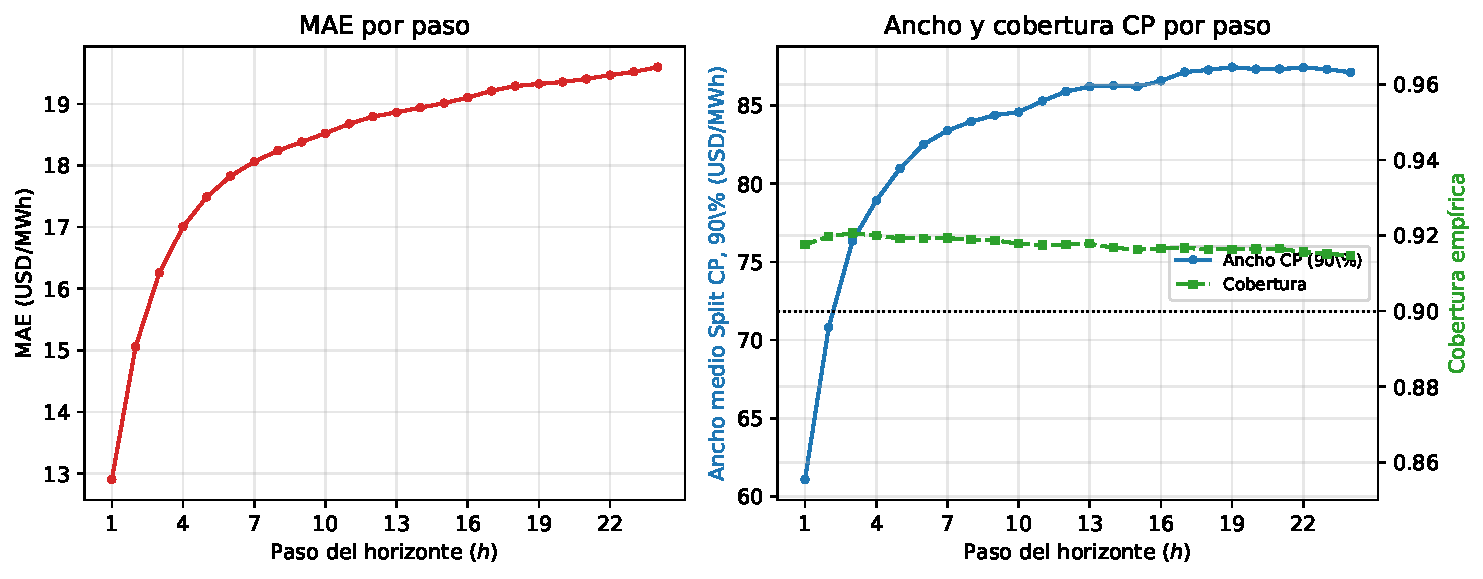
\includegraphics[width=0.92\textwidth]{fig_h24_mae_ancho.pdf}
    \vspace{0.2em}
    \footnotesize
    \begin{itemize}
        \item El MAE crece 52\% del primer al último paso; en promedio, el modelo no supera a la persistencia diaria (11 de 16 combinaciones).
        \item La cobertura de Conformal Prediction se mantiene en 0.915--0.921 (90\% nominal) en los 24 pasos, y el ancho se estabiliza desde el paso $\sim$12.
    \end{itemize}
\end{frame}

\begin{frame}{¿Se mantienen las conclusiones a 24 horas?}
    \footnotesize
    \begin{table}
        \centering
        \begin{tabular}{p{3.1cm}p{5.3cm}p{2.7cm}}
            \toprule
            \textbf{Conclusión a 1 hora} & \textbf{Resultado a 24 horas} & \textbf{¿Se mantiene?} \\
            \midrule
            Heterocedasticidad horaria del error & Levene significativo en los 24 pasos en 7 de 8 barras (Charrúa se debilita) & Sí \\
            \addlinespace
            LW-ACP es el mejor método de CP & Menor Winkler en los 24 pasos; intervalos 17.2\% más angostos que Split CP & Sí, más fuerte \\
            \addlinespace
            LayerNorm supera a DyT & Diebold-Mariano: LN gana en 1 barra, 7 empates & No: equivalentes \\
            \addlinespace
            S+C supera a P+C & P+C gana en 3 barras, S+C en 2, 3 empates; P+C 4\% menos MAE & No; S+C más simple \\
            \bottomrule
        \end{tabular}
    \end{table}
    \vspace{0.3em}
    \begin{itemize}
        \item Lo que traspasa al \textit{day-ahead} es la estructura del error y la cuantificación de incertidumbre; la ventaja en precisión puntual, no.
    \end{itemize}
\end{frame}

\begin{frame}{¿Por qué P+C mejora a 24 horas?}
    \footnotesize
    \begin{columns}[T]
        \column{0.48\textwidth}
        \textbf{Qué información comparten} ($R^2$ al reconstruir Prophet desde la posición solar)
        \begin{table}
            \centering
            \begin{tabular}{lr}
                \toprule
                \texttt{daily}  & 0.82--0.89 \\
                \texttt{yearly} & 0.49--0.68 \\
                \texttt{weekly} & 0 \\
                \texttt{trend}  & $\le 0$ \\
                \bottomrule
            \end{tabular}
        \end{table}
        La posición solar ya contiene la hora del día, pero no el día de la semana ni el nivel de largo plazo.
        \column{0.48\textwidth}
        \textbf{En qué se apoya el modelo} (promedio 8 barras)
        \begin{table}
            \centering
            \begin{tabular}{lrr}
                \toprule
                & 1 h & 24 h \\
                \midrule
                \texttt{y\_real} en encoder S+C & 66\% & 29\% \\
                \texttt{y\_real} en encoder P+C & 49\% & 22\% \\
                \texttt{weekly} en decoder P+C  & 11\% & 18\% \\
                \bottomrule
            \end{tabular}
        \end{table}
    \end{columns}
    \vspace{0.4em}
    \begin{itemize}
        \item A 1 hora mandan el precio reciente y la hora del día, que ambas estrategias tienen: S+C gana por simplicidad.
        \item A 24 horas el precio reciente pierde peso y P+C recurre al día de la semana, que solo él conoce.
        \item Propuesta: un único TFT con posición solar + \texttt{weekly} + \texttt{trend}.
    \end{itemize}
\end{frame}

\begin{frame}{Extensiones exploradas}
    \begin{itemize}
        \item \textbf{Piloto sin recorte de outliers}: a $h=1$, en las ocho barras, no perjudica el MAE general y reduce los errores más grandes (error máximo menor en las 8 barras, MAE en el percentil 99 menor en 7); significativo individualmente solo en 2 barras. Resultado mixto a $h=24$ (4 barras).
        \item \textbf{Granularidad temporal}: mayor resolución (15 min) mejora la capacidad predictiva de forma consistente, controlando por período histórico.
        \item \textbf{Sensibilidad a pérdida asimétrica}: la ventaja de S+C-LN se sostiene en 7 de 8 barras independientemente de qué error sea más costoso.
    \end{itemize}
\end{frame}

% ============================================================
\section{Conclusiones}

\begin{frame}{Conclusiones principales}
    \begin{enumerate}
        \item \textbf{La estrategia más simple es la más precisa a una hora}: S+C supera a P+C, con la posición solar dominando el decoder del TFT; a 24 horas P+C es algo más preciso (4\%), y S+C queda cerca con un solo modelo.
        \item \textbf{LW-ACP} combina ponderación horaria y adaptación \textit{online}, logrando el mejor Winkler y pinball al 90\% con cobertura calibrada, y los intervalos más angostos al 95\%.
        \item Los errores más extremos siguen un patrón mecanístico común (desfase de fase de $\sim$1h), no ruido aleatorio disperso.
        \item A una hora supera a la literatura reciente de ML clásico al mismo horizonte; a 24 horas la calibración de los intervalos se mantiene, pero la predicción puntual no supera a la persistencia.
        \item Puerto Montt permanece como un caso no resuelto, estructuralmente distinto al resto del SEN.
    \end{enumerate}
\end{frame}

\begin{frame}{Limitaciones}
    \begin{itemize}
        \item \textbf{Horizonte}: los resultados principales son a una hora; a 24 horas la predicción puntual no supera a la persistencia diaria.
        \item Un único split cronológico entrenamiento/validación/prueba (no \textit{walk-forward validation}) por costo computacional.
        \item Sin semilla fija para los modelos principales del Capítulo 4 (sí para el estudio de robustez).
        \item Esfuerzo de ajuste de hiperparámetros asimétrico entre Prophet (optimizado por barra) y TFT (fijo).
        \item Reproducibilidad parcial del entorno de entrenamiento en GPU (versiones de librerías del cluster no registradas).
        \item Pipeline no directamente desplegable en operación real: ERA5 se publica con rezago.
    \end{itemize}
\end{frame}

\begin{frame}{Trabajo futuro}
    \begin{itemize}
        \item Mejorar el \textit{day-ahead} con información conocida de antemano, por ejemplo el costo marginal programado del CEN como variable de entrada.
        \item Comparar LW-ACP contra AgACI (agregación de múltiples $\gamma$ vía expertos \textit{online}).
        \item Extender la comparación contra el CEN a Atacama y Tarapacá.
        \item \textit{Walk-forward validation} sobre múltiples ventanas rodantes.
        \item Investigar directamente el mecanismo del desfase de fase (pérdida que penalice error de temporización).
        \item Extender el estudio de granularidad a las ocho barras y el piloto de outliers a las ocho barras a $h=24$.
        \item LW-ACP con adaptación \textit{online} indexada por hora del día.
    \end{itemize}
\end{frame}

\begin{frame}
    \centering
    \Huge Gracias

    \vspace{1em}
    \normalsize
    \url{github.com/benjamitchell/Tesis-TFT-Electricidad}
\end{frame}

\end{document}
